% Detail what notes were taken when reading the code and what was noticed from afar
% We should say that reading the code is not great in that it usually focuses our testing on some things and push us not to test, things that 
% we expect to be correct (given we know the implementation). As such, it is always better to try and make no assumptions about the contents 
% of the code when writing the tests. 
% =========================================================================

% --------------
% Code structure 
% --------------
% 1 - Assess the structure of the code.
\subsection{Code Structure} 
Overall, the code is difficult to read in part due to the lack of coherence and consistency with the coding style and the lack of useful documentation, but mainly due to questionable implementation choices. 

Below, we shall focus on the code's structure and testability. Critique of the code that is unrelated to its testability can be found in Appendix \ref{appendix:code-read} [and in \ref{sec:code-style}]. 

\begin{itemize}
	\item We note that error reporting in the application is weak: no exceptions thrown anywhere, none of the implemented methods return booleans or integers that could report errors (like returning -1 to indicate an error). There are no means by which  to valid errors occurrences in methods, such as when the ID provided in the delete method is not owned by any customer. 
	\item There are many instances of duplicated code that should have been separated in a private method to be called by others (deleteCustomer, updateCustomer) all attempt to find a customer with the given ID. 
\end{itemize}

% -----------------------------------
% Code testability & Recommendations  
% -----------------------------------
% 2 - Comment on its testability 
\subsection{Code testability \& Recommendations}

The below items have been identified as hindrances to our testing. Each item will be described and suggestions to improve the structure provided. 

\subsubsection{Thread-safety}
The design of Main does not accomodate many threads running simultaneous versions of the application, not least because AllCustomers and Scanner are static, making them shared resources. AllCustomers houses most - if not all - of the Customer data structures, which also becomes shared by all Threads. This will inevitably lead to race conditions. 
\par 
To overcome this and allow for many Main instances to be spawned simulatenously without conflicting with each other's state, we 
\begin{itemize}[noitemsep]
	\item remove static modifiers from the class's members and methods.  
	\item add a default constructor.
	\item update the \lstinline{main} method to instantiate Main, via \lstinline{Main main = new Main();}.
	\item switch to making method calls on the instance rather than static methods. 
\end{itemize}
The above steps improve encapsulation of state within Main instances and reduce the number of shared resources between threads, but are not sufficient. There are one of each standard input and output shared by all threads, below we describe how we get around these being shared. 

% -------------------------------------------------------
\begin{minipage}[b]{0.5\textwidth}
\begin{figure}[H]
\centering
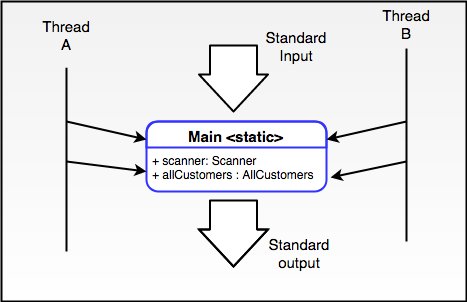
\includegraphics[scale=0.4]{res/STE-Page-1-original.png}
\caption{Before changes: one static Main}
\end{figure}
\end{minipage}
% -------------------------------------------------------
\begin{minipage}[b]{0.5\textwidth}
\begin{figure}[H]
\centering
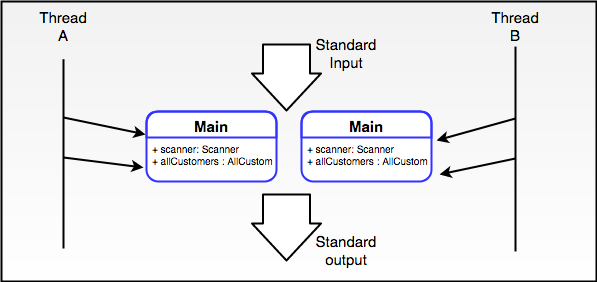
\includegraphics[scale=0.4]{res/STE-Page-2-original.png}	
\caption{After changes: different instances of Main}
\end{figure}
\end{minipage}
% -------------------------------------------------------

\subsubsection{Main: Standard I/O}
\label{sec:main-stdio}
The application, being command-line driven, relies on stdin for user input and stdout for output. Testing the software in a behaviour driven methodology necessitates injecting input to stdin to simulate user input and inspecting the output from stdout to verify correctness. 
\par
To validate the output of the application, the tester needs to redirect stdout somewhere where they can get a the string of the output and inspect it. A quick solution to this, and one that does not require any code changes on behalf of the application under test, is to call \lstinline{System.setOut(printStream)} prior to the start of the tests; this effectively redirects all output which would have otherwise gone to stdout into the printStream; which can then be used by the tester for checking. 
\par
The problem with this approach is that System.in is shared by all components of the Java executable which in a test environment includes the test suite as well as all instances of the application being tested (Main in this case). Recall that test suites often run test methods in parallel; this can lead to multiple Main instances running simultaneously and appending output to the same stream. Even worse is that the Cucumber-JVM shares the same stdout and may choose to output its debug info or test results to it as well. 
\par 
\textbf{Recommendation}: To isolate the standard input and output of each Main instance and facilitate testing, we can introduce class members of type PrintStream and InputStream in Main class and allow callers to Main's constructor to inject those streams.
\par
This allows us to provide specific streams for Main to work with when running the instance in a test environment where we would like to exert control and inspect the streams. 
\par 
Following our changes, creators of Main can either choose to provide their own streams or stick to the default stdin and stdout by calling Main's default constructor. 
\par
Another class in the application uses System.out to print and that is AllCustomers. It was debated whether we should dependency inject the streams to print to as well, but as there exists only one method concerned with printing in AllCustomers: `printCustomers`, it was decided that adding another \lstinline{printCustomers} method taking in a PrintStream would suffice.
% We would encourage considering a software redesign, limiting the span of objects that may write to stdout or read from stdin. [ Can expand on this more? ]
\par
\begin{figure}
\begin{lstlisting}
/**
 * Stream to write application's output to, defaults to System.out.
 */
private final PrintStream out;

/**
 * InputStream to be used for reading user input, defaults to System.in
 */
private final InputStream in;

/**
 * default constructor
 */
public Main() {
    this(System.in, System.out);
}

/**
 * constructor taking in the InputStream and PrintStream to be used
 * @param in InputStream to read from
 * @param out PrintStream to write to
 */
public Main(InputStream in, PrintStream out) {
    this.in = in;
    this.out = out;
}
\end{lstlisting} 
\ref{code:snippet-1}
\end{figure}

\subsubsection{Stopping Main more gracefully}
(1) method call 
(2) do not invoke System.exit(2) 
% * Allow for Main's start/stop execution to be controlled via methods. Currently, to stop main, the user must press 'q' which then leads to System.exit(). If running a test suite, this will cause the whole test suite to exit. We replace System.exit() with logic that causes the method to return. 
 % -	In a normal running App,   when the method returns, the app will reach the end of Main and exit naturally (and gracefully), when run under a test suite, the framework will continue to run after the method has returned which is what we wanted in the first place. 
 %  - Add method `stop()` and member field `running` which when set to false causes the User Input loop to exit, leading to stop of the program.

\begin{itemize}
	 \item Customer ID on creation, also expose getCustomer() 
	 % print the ID of the created Customer otherwise there is no way to know how to list that specific customer. (see newCustomer, has the 'id' of the new customer printed.)
	 % add method getCustomer in Main to aid with testing. As we would prefer getting the customer object from main directly rather than going through the route of listing customers with that ID, and serializing a customer object from the printed fields to use in our tests. e.g. adding "Sami Farhat TB1000 10000", then the ID is output, the we would have to, use 'l' <id>, and get the output from the program and serialise a Customer object from the output. Also, a bug in the listing would cause all tests depending on getting a customer from the database to fail. To separate the tests better, we create a method in Main that returns a customer object directly from the data structure in AllCustomers given a CustomerID. 

	 % TODO: check what changes I've made to other classes????
	 % TaxEngine mostly for unit testing. Were there any changes due to BDD

	 \item TaxEngine contains one bulky method `taxAmount` that does all computations in a single method. 
	 %This means that it would be difficult to write unit tests that could help narrow down where the error in tax computation occurs when / if they occur. 
	 %For instance, it would be more apt to separate the parsing of the tax code from the calculation of the tax required. 

\end{itemize}


 % ============================================================================

* There is a very clear lack of documentation accross the source code. Methods do not have javadoc, most method implementations do no supply them either excepting for a few inline comments. 

* there's no code style consistency: 
	- some methods put spaces between open bracket and first param and closing bracket and last parameter. Other methods do not obey this. 
	- some methods use canonical camel case while others break this (newcustomer vs. addCustomer)
	- Implementation oddities, as if the developer is not familiar with Java programming: 
		* `String name = new String()` is not often seen as it is sufficient to use `String name = "";' which is equivalent
		* int i = 0; then using for(i=0; i < n; i++). As i is not used outside of the loop, it does not need to be defined outside. 
	- AllCustomers is a badly named class, CustomerManagement is a better alternative. 
	- 

AccountNumbers
--------------
Is not a well implemented Singleton pattern because the constructor is made protected and not private, meaning other classes in the same package can still instantiate it.


AllCustomers
------------
* method getCustomer() returns a Customer object that has an "INVALID\_ID" when no such customer is present. This is unusual in that most common implementations would either throw an exception or return null. This implementation would be fine and accepted were it to be more documented. 


* updateCustomerXXXXX: all of these methods start off finding the customer, we should create a private method that returns the customer for a given ID. Also, discussing the current implementation of finding that customer; the below: 

\begin{lstlisting}	
	int i = 0;
	int intCustomerIndex = 0;
	
	boolean blFound = false;

	for (i=0; i< intCurrentCustomerIndex; i++) {
		if (customers[i].getAccountNum() == intCustomerID) {
			blFound = true;
			intCustomerIndex = i;
			break;
		}
	}
	if (blFound == true) {
		customers[intCustomerIndex].setfirstName( strFirstName);
	}
\end{lstlisting}
can be written as below: 
\begin{lstlisting}
int intCustomerIndex = -1;
for (int i=0; i< intCurrentCustomerIndex; i++) {
	if (customers[i].getAccountNum() == intCustomerID) {
		intCustomerIndex = i;
		break;
	}
}
if (intCustomerIndex != -1) {
	customers[intCustomerIndex].setfirstName( strFirstName);
}
\end{lstlisting}

* method deleteCustomer() 
why not just place `customers[i] = customers[i+1];` in the first if? 

Main
-----

* A new instance of AllCustomers is created every time IntepretCommand is run(), which happens everytime some form of exception is thrown, because that's the only way to break out of the `while(true)` loop in InterpretCommand. 

* String lineSeparator is useless. Totally useless.
